\section{Compressione video}
La compressione video deve necessariamente essere lossy, dato che la quantità di ridondanze è generalmente elevata e le dimensioni dei video non compresse sono ingestibili dai supporti di memoria. Il tipo di processing adottato è \textbf{intra-frame} o \textbf{inter-frame}. 

Ci sono soluzioni che considerano solo la ridondanza spaziale o temporale, e altre che sfruttano la ridondanza percettiva attraverso le limitazioni del sistema visivo/uditivo. 

Il procedimento più semplice applica codifiche predittive oppure JPEG frame per frame, ma queste tecniche sono legate solo alle caratteristiche spaziali: esse devono essere estese valutando anche la \textbf{ridondanza temporale}, in termini di differenze tra i frame con predizioni (istogramma piccato).

Il primo step è naturalmente la differenza tra frame consecutivi, a cui è associata un'entropia: ciò funziona in modo ottimale quando le zone delle immagini cambiano poco, ma non è efficace quando la camera non è perfettamente ferma, o ci sono cambi di luce, o le scene sono in movimento.

Generalmente anche in presenza di queste condizioni c'è correlazione, ma se la differenza tra due fotogrammi è il rumore o è dovuta al cambio di scena il segnale è poco correlato. In alcuni casi è possibile predirre anche il movimento.

\subsection{Motion compensation}
La \textbf{motion compensation} è una codifica predittiva che consiste nella stima dei vettori di moto con cui le porzioni di frame vengono spostati, e nella loro applicazione per le variazioni future. 

Lo scopo è l'individuazione e la compensazione del moto, studiando il disallineamento dei pixel. La stima riguarda gli spostamenti dei macro blocchi 16$\times$16, ma questa tecnica non funziona in caso di differenze significative.

Per semplificare il procedimento, si distinguono alcune tipologie di frame:
\begin{itemize}
	\item Target frame, da codificare;
	\item Reference frame, utilizzato per il calcolo delle differenze;
	\item I-frame (intra/independent frame, compressi con JPEG), frame di partenza per la predizione;
	\item P-frame, risultato della codifica, che può essere:
	\begin{itemize}
		\item Predetto solo in base al reference frame;
		\item Predetto in base al frame precedente e ai frame successivi. 
	\end{itemize}
\end{itemize}
Il disallineamento fra il reference frame e il target è chiamato MV (Motion Vector). Utilizzare le informazioni dei frame consecutivi aumenta la precisione.

Ogni gruppo non sovrapposto di pixel viene assegnato a un vettore di moto comune. L'intensità è 16, con 8 canali cromatici ($\nicefrac{1}{4}$) per semplificare il campionamento $4 : 2 : 0$. 

Dato un macroblocco del target frame, viene cercato \textbf{il più simile} macroblocco nel reference frame tra i precedenti e successivi. Le dimensioni della finestra di ricerca variano in base allo standard utilizzato. Il MV consiste nelle sottrazioni, espresse tramite coppie di valori sugli assi.

L'encoder calcola la somiglianza tra il frame predetto e quello ottenuto, detta \textbf{motion compensated difference frame} $MCD(n)$. MCD ha una correlazione fra pixel inferiore a quella risultante dalla differenza tra target e difference.

Il decoder prende in input MCD, il frame reference e i vettori di moto, per ricostruire il frame predetto e in seguito il frame target, con perdita. I blocchi predetti sono organizzati su una griglia, al contrario di quelli utilizzati per la predizione.

Le possibilità per la compressione sono la \textbf{codifica} della differenza oppure la \textbf{compensazione} della differenza attraverso il moto. 

Riassumendo:
\begin{enumerate}
	\item Individuazione del target frame;
	\item Scorrimento dei macroblocchi e ricerca del più simile al blocco del reference frame, cercando il vettore di moto;
	\item Sostituzione con il più simile traslato di un vettore di moto (compensazione);
	\item Calcolo della differenza tra predizione e target (errore);
	\item Codifica della differenza.
\end{enumerate}

La compensazione del moto viene applicata in modo efficiente ai canali di luminanza, mentre i valori di crominanza sono meno correlati: i vettori di moto si ottengono sottocampionando i risultati sulla luminanza.

\begin{figure}[h]
	\centering
	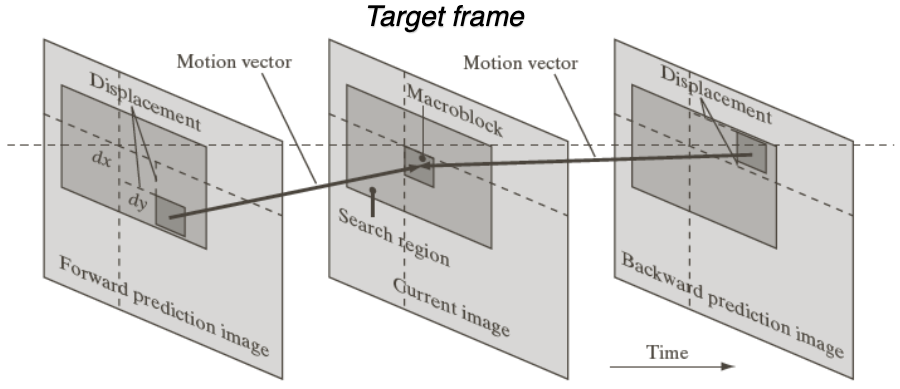
\includegraphics[scale=0.4]{Lezioni/Immagini/motion-estimation}
\end{figure}

Se il moto è da sinistra verso destra, le zone di sinistra hanno l'errore di predizione più alto perché sono zone che non esistono nei frame precedenti.

Il vettore di moto di ciascun macroblocco è calcolato trovando nel reference frame la posizione più probabile di quel macroblocco del target frame: il reference frame può essere tra i precedenti o i successivi. Un frame codificato usando entrambi si indica come B-frame (bidirectional).

La posizione più probabile è quella che minimizza una misura di errore tra reference e target, all'intorno della regione definita.

Si definisce MAD la distorsione media assoluta tra pixel di due macroblocchi di dimensioni $N \times N$ disallineati, da minimizzare.

La stima del moto con frame successivi implica un ritardo nei calcoli finché le informazioni sono incomplete. Per semplificare le operazioni, la ricerca del macroblocco è effettuata in un intorno, e non ha standard definiti:
\begin{itemize}
	\item Ricerca logaritmica, valutando la MAD su 9 punti (3$\times$3), selezionando il più vicino e dividendolo a sua volta, fino ad arrivare a un errore tollerabile, nonostante il rischio di concentrazione sui punti locali tralasciando il possibile ottimo globale;
	\item Multirisoluzione, in tre passi;
	\begin{enumerate}
		\item Stima iniziale sul frame a risoluzione minore;
		\item Raffinazione a risoluzione intermedia;
		\item Determinazione del vettore di moto finale sulla risoluzione massima.
	\end{enumerate}
\end{itemize}

\subsection{Standard per la codifica}
Gli standard di codifica video digitale sono regolati da:
\begin{itemize}
	\item ITU (raccomandazioni), con un carattere generale e orientato alle applicazioni real-time (H.xx);
	\item ISO, MPEG e derivati, per necessità più ampie come storage e broadcast.
\end{itemize}

Gli IP frames sono particolari sequenze di frame, la cui combinazione è la base di H-261:
\begin{itemize}
	\item I (intra) servono per predirre i frame successivi, codificati con JPEG con riduzione della ridondanza e DCT;
	\item P (picture), codificati tramite MC e predizione, e in seguito DCT insieme al vettore di moto.
\end{itemize}
La sequenza è I-P-P, con finestra temporale stabilita dall'encoder e disallineamento misurato in pixel.

Nella quantizzazione per coefficienti DCT, non vengono applicate matrici di quantizzazione ma si usa una costante per tutti i coefficienti, calcolata per approssimazione tra DCT e step-size.

Il rapporto di compressione è più alto perché questa metodologia non sfrutta solo la ridondanza spaziale, ma riduce anche quella temporale. I frame B sono quelli su cui la perdita è maggiore, perché vengono codificati agendo su entrambe le direzioni.

Non sempre i macroblocchi sono codificati nello stesso modo: a seconda del tipo di frame e dell'errore di predizione essi saranno determinati diversamente. Se nessuna strategia è la migliore, si utilizza l'interpolazione.

\subsubsection{MPEG}
\textbf{MPEG} (Motion Picture Experts Group) è uno standard creato da ISO per la codifica di informazioni audio e video in formato digitale compresso, con bitstream predefiniti. 

MPEG-1 è il primo standard per i filmati digitali, non interlacciato. I blocchi hanno dimensioni 8$\times$8, e l'unità elementare di codifica è il macroblocco 16$\times$16.

\begin{figure}[h]
	\centering
	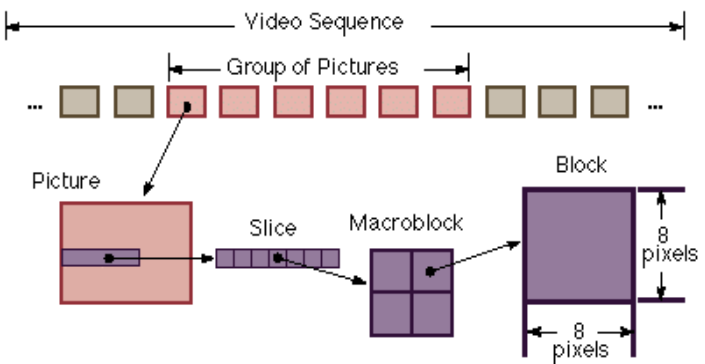
\includegraphics[scale=0.4]{Lezioni/Immagini/mpeg-gerarchica}
\end{figure}

I dati hanno una \textit{struttura gerarchica}:
\begin{itemize}
	\item Più macroblocchi formano una \textbf{slice}, codificata in modo indipendente con differenti fattori di scala, senza propagazione dell'errore;
	\item Un'immagine del frame codificato consiste in una \textbf{picture};
	\item Più pictures sono definite \textbf{GOP};
	\item Più GOP sono inclusi in una \textbf{sequence}.
\end{itemize}

La predizione è solamente di tipo forward, e ci sono casi in cui il frame precedente non è sufficiente per una buona stima del vettore di moto: si introduce \textit{backward prediction}.

 \begin{wrapfigure}{R}{0.4\textwidth}
	\vspace{-10pt}
	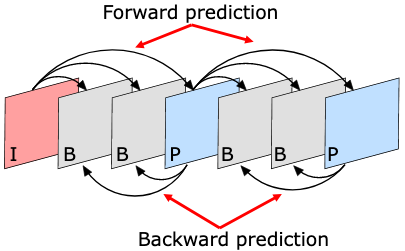
\includegraphics[width=0.4\textwidth]{Lezioni/Immagini/ibp}
	\vspace{-30pt}
\end{wrapfigure}

Analogamente a IP, lo standard MPEG definisce tre tipi di picture:
\begin{enumerate}
	\item I, codificate sfruttando la ridondanza;
	\item P, codificati con predizione compensata del moto rispetto al picture precedente;
	\item B, codificati con predizione compensata del moto rispetto al picture precedente, successivo o entrambi (buffering).
\end{enumerate}

Per ogni B-frame sono calcolati due vettori di moto per ogni macroblocco: se il matching è buono, viene fatta una media delle predizioni. La compressione di I è peggiore, mentre B ha priorità minore ma compressione maggiore.

Non sempre i macroblocchi sono codificati allo stesso modo: l'encoder sceglie l'approccio più adatto in base all'informazione contenuta.
\begin{itemize}
	\item I sono intra-coded, con matrice di quantizzazione variabile;
	\item P sono codificati come intra se non è possibile avere una predizione sufficientemente accurata;
	\item B sono determinati dal precedente, dal successivo o dalla media, a seconda dell'errore di predizione.
\end{itemize}

\begin{figure}[h]
	\centering
	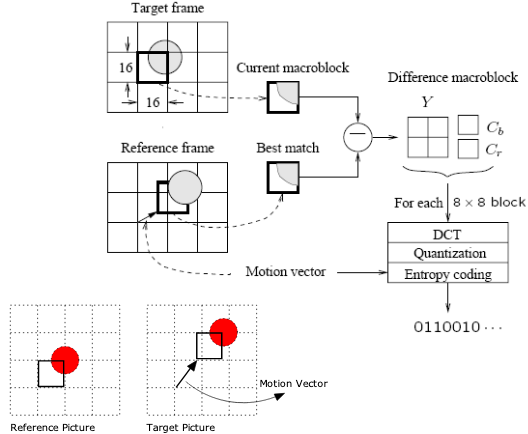
\includegraphics[scale=0.7]{Lezioni/Immagini/p-frame}
\end{figure}

\subsection{Versioni di MPEG}
MPEG-2 è un'evoluzione di MPEG-1, con la stessa struttura base ma dedicato a video di qualità superiore, con bitrate maggiori di 4 Mbps. Questo standard implementa diverse misure di adattabilità con livelli di decodifica in base ai frame rate, pertanto è più scalabile.

Le versioni sono a qualità variabile, trattando i coefficienti secondo la perdita indicata. I video sono interlacciati, gestendo i field (righe dispari e pari), ottenendo un errore più basso. L'approccio può essere frame prediction o field prediction, codificando top e bottom separatamente con due vettori di movimento.

\begin{figure}[h]
	\centering
	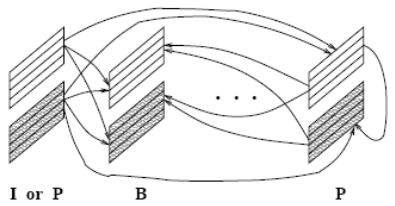
\includegraphics[scale=0.7]{Lezioni/Immagini/ipbp}
\end{figure}

L'utilizzo dei field ha un effetto diretto sulla quantizzazione: il campo è 16$\times$8, il pattern a zig-zag è opzionale e sono ammessi anche pattern alternativi. Il sottocampionamento è solo in una dimensione, essendo i sottoinsiemi incorrelati. 

Non tutti i livelli ammettono le stesse variazioni: esse cambiano in base alla dimensione e i frame al secondo, campionando con diversi profili di chroma. 

Il concetto di scalabilità prevede alcune caratteristiche:
\begin{itemize}
	\item Livelli base a qualità inferore;
	\item Livelli base indipendenti per fornire un video di qualità inferiore;
	\item Codifica e decodifica dei livelli superiori dipendenti dai precedenti.
\end{itemize}

I layers sono definiti in base ad alcune possibilità di codifica:
\begin{itemize}
	\item SNR, con differente quantizzazione a seconda del livello;
	\item Scalabilità spaziale, dividendo i dati relativi alle immagini sotto-campionati da quelli che permettono di ricostruire l'immagine completa;
	\item Temporale;
	\item Partizionamento dei dati con le frequenze.
\end{itemize}
Questi modi possono eventualmente essere combinati in una scalabilità ibrida.

MPEG-4 pone l'attenzione sull'\textit{interattività con l'utente}, introducendo ulteriori caratteristiche basate sugli oggetti e le loro relazioni (anche tridimensionali). La trasmissione è possibile anche su mezzi a banda limitata, garantendo efficienza e accesso universale.

Esistono anche possibili oggetti precodificati, come le animazioni che permettono di inserire effetti speciali nei video. Ogni oggetto può essere trasmesso in uno stream separato, ed essi sono ricomposti dopo la decodifica.

\begin{figure}[h]
	\centering
	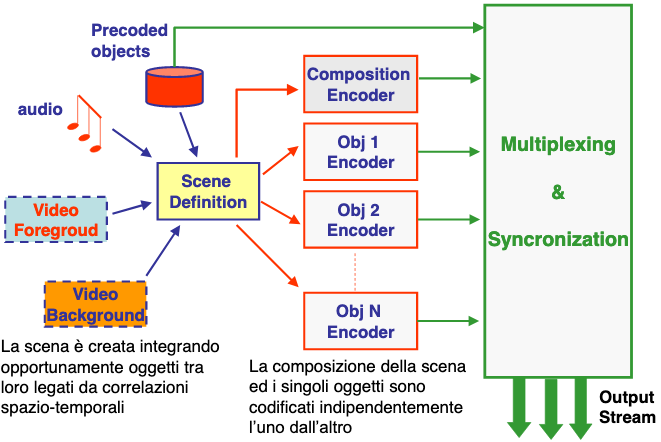
\includegraphics[scale=0.6]{Lezioni/Immagini/mpeg-4}
\end{figure}

Tutti i componenti di una presentazione sono accessibili tramite Object Descriptors, posti in mutua relazione tramite scene description e relative informazioni spazio-temporali. La ricostruzione è possibile grazie a BiFS, linguaggio di descrizione.

Alcuni standard di decompressione introducono un filtro di denoising, applicato dopo la decodifica per rimuovere gli artefatti di blocchettizzazione. 

MPEG-7 definisce gli strumenti necessari per descrivere il contenuto audiovisuale dei dati multimediali e consentire l'interoperabilità tra diversi sistemi e applicazioni. 

Permette la migliore gestione, distribuzione e fruizione delle descrizioni, aiutando utenti e applicazioni ad identificare e filtrare le informazioni rilevanti.

Ogni scena viene caratterizzata e classificata secondo un numero di features che impongono un grado di \textbf{correlazione tra gli oggetti}, tramite sintassi e semantica.

Ogni \textit{descrittore} è una rappresentazione di una feature, per caratteristiche di basso livello. Può essere atomico o composito, e ogni feature può averne uno o più.
